% ============================================================
%  Online Learning - Adaptive Hedge
%  Machine Learning Project Report
%  University of Milan, A.Y. 2025/26
%  Instructor: Prof. Nicolo Cesa-Bianchi
% ============================================================

\documentclass[11pt,a4paper]{article}

% ---- Packages -----------------------------------------------
\usepackage[margin=2.5cm]{geometry}
\usepackage{amsmath,amsthm,amssymb}
\usepackage{bm}
\usepackage{graphicx}
\usepackage{subfig}
\usepackage{booktabs}
\usepackage{hyperref}
\usepackage{xcolor}
\usepackage{microtype}
\usepackage{parskip}
\usepackage{enumitem}
\usepackage[T1]{fontenc}
\usepackage{lmodern}

% ---- Hyperref setup -----------------------------------------
\hypersetup{
    colorlinks = true,
    linkcolor  = blue!60!black,
    citecolor  = blue!60!black,
    urlcolor   = blue!60!black,
}

% ---- Theorem environments -----------------------------------
\newtheorem{theorem}{Theorem}
\newtheorem{lemma}[theorem]{Lemma}
\newtheorem{definition}[theorem]{Definition}

% ---- Math shorthands ----------------------------------------
\newcommand{\E}{\mathbb{E}}
\newcommand{\R}{\mathbb{R}}
\newcommand{\wt}{\boldsymbol{w}_t}
\newcommand{\bsl}{\boldsymbol{\ell}}
\newcommand{\Lstar}{L_T^*}
\newcommand{\Rhat}{R_{\mathrm{AdaHedge}}}
\newcommand{\dt}{\delta_t(\eta)}
\newcommand{\DT}{\Delta_T(\eta)}
\newcommand{\bud}{b(\eta)}

% ---- Title block --------------------------------------------
\title{%
  \textbf{Online Learning with Adaptive Hedge} \\[4pt]
  {\large Assignment 1: Statistical Methods for Machine Learning} \\[2pt]
  {\normalsize University of Milan, A.Y.\ 2025/26}
}
\author{%
  SeyedSina SajadiMorafah
}
\date{June 2026}

% ---- Spacing adjustments for floats -------------------------
\setlength{\textfloatsep}{10pt plus 2pt minus 2pt}
\setlength{\floatsep}{8pt plus 2pt minus 2pt}
\setlength{\intextsep}{10pt plus 2pt minus 2pt}
\setlength{\abovecaptionskip}{6pt}

% =============================================================
\begin{document}
\maketitle
\thispagestyle{empty}

% ---- Plagiarism Declaration (verbatim, as required) ---------
\begin{center}
\fbox{%
  \begin{minipage}{0.92\textwidth}
    \small
    \textbf{Plagiarism Declaration} \\[4pt]
    I declare that this material, which I now submit for assessment, is entirely
    my own work and has not been taken from the work of others, save and to the
    extent that such work has been cited and acknowledged within the text of my
    work. I understand that plagiarism, collusion, and copying are grave and
    serious offences in the university and accept the penalties that would be
    imposed should I engage in plagiarism, collusion or copying. This assignment,
    or any part of it, has not been previously submitted by me or any other person
    for assessment on this or any other course of study.
  \end{minipage}
}
\end{center}

\vspace{1em}

% =============================================================
\begin{abstract}
Hedge is a classic algorithm for prediction with expert advice, but it needs a
learning rate fixed in advance. Pick it wrong and the algorithm either reacts
too slowly to an easy problem or too fast to a hard one. This report studies
AdaHedge, which removes that requirement. It watches a quantity called the
mixability gap and switches to a smaller rate once the gap uses up its budget.
I implemented both algorithms from scratch in Python, built three synthetic
loss sequences (stochastic, adversarial, and low-gap stochastic) following the
setup in van Erven et al. (NeurIPS 2011), and compared AdaHedge against five
fixed learning rates.

In the stochastic regime one expert is clearly better than the rest, so
AdaHedge never needs to change its rate. It stays at $\eta=1$ for all
10{,}000 rounds and ends with a regret of $2.28$, exactly matching fixed Hedge
at $\eta=1$. In the adversarial regime, where the best expert swaps halfway
through, AdaHedge again uses a single rate the whole time and ends well
inside its worst-case bound: regret $1.72$ against a bound of $313.13$
(Theorem~5). The low-gap regime is the interesting one. The gap between
experts is only $0.01$, so AdaHedge needs five segments before it settles
down. Its final regret is $60.06$, slightly worse than plain fixed Hedge at
$\eta=1.0$ or $\eta=0.5$ on this run. That is not a bug and not a broken
guarantee: Theorem~5 only promises AdaHedge stays under $440.49$ here, and it
does, with room to spare. It is simply a reminder that a constant-regret
guarantee describes the worst case. It does not promise a win against every
other method on every single run.
\end{abstract}

\clearpage
\tableofcontents
\clearpage

% =============================================================
\section{Problem Statement and Theory}
\label{sec:theory}

\subsection{The Online Learning Setup}

We consider the \emph{prediction with expert advice} framework.  Time unfolds in
discrete rounds $t = 1, 2, \ldots, T$.  At the start of each round, the learner
chooses a probability distribution $\wt = (w_t^1, \ldots, w_t^K)$ over $K$
experts.  The environment then reveals a loss vector
$\bsl_t = (\ell_t^1, \ldots, \ell_t^K) \in [0,1]^K$, and the
learner incurs the expected loss
\[
  \wt \cdot \bsl_t = \sum_{k=1}^{K} w_t^k \, \ell_t^k.
\]
There is no probabilistic model for the losses. The sequence can even be
chosen by an adversary who wants the learner to fail.

After $T$ rounds, expert $k$ has accumulated loss $L_T^k = \sum_{t=1}^T \ell_t^k$.
The learner wants to minimise its \emph{regret}:
\begin{equation}
  \label{eq:regret}
  R(T) = \sum_{t=1}^T \wt \cdot \bsl_t \;-\; \Lstar,
  \qquad \Lstar = \min_{1 \le k \le K} L_T^k.
\end{equation}
Regret is how much worse the learner does than the single best expert in
hindsight. A sub-linear guarantee, $R(T) = o(T)$, means the learner catches
up to the best expert on average as $T$ grows.

\subsection{The Hedge Algorithm}

The Hedge algorithm (Freund and Schapire, 1997) assigns weights to experts
proportionally to their exponentiated cumulative losses.  Starting from a uniform
prior $w_1^k = 1/K$, the weight update after round $t$ is:
\begin{equation}
  \label{eq:hedge_update}
  w_{t+1}^k = \frac{\exp(-\eta \, L_t^k)}{\sum_{k'} \exp(-\eta \, L_t^{k'})},
  \qquad \eta > 0.
\end{equation}
The parameter $\eta$ is called the \emph{learning rate}.  A large $\eta$ makes
the algorithm react sharply to differences in cumulative losses, which helps when
one expert is clearly better than the rest.  A small $\eta$ keeps the distribution
closer to uniform, which is safer in adversarial settings where no single expert
is reliably good.

The key regret bound for Hedge follows from bounding the log of the normalisation
constant.  When $T$ is known in advance and $\eta$ is set to
$\eta^*(T) = \sqrt{8 \ln K / T}$, the resulting regret satisfies
\begin{equation}
  \label{eq:hedge_bound}
  R_{\mathrm{Hedge}}(T) \le \sqrt{\tfrac{T \ln K}{2}}.
\end{equation}
This bound is worst-case optimal, up to constants, over every possible loss
sequence. But it never gets better just because the sequence turns out to be
easy. If $\Lstar$ were known ahead of time, setting
$\eta^*(L^*) = \ln\!\left(1 + \sqrt{2\ln K / \Lstar}\right)$ gives the tighter
bound $\sqrt{2 \Lstar \ln K} + \ln K$. The problem is that neither $T$ nor
$\Lstar$ is known before the game starts.

This is the real difficulty: a fixed rate has to guess how hard the sequence
will be before seeing a single loss. That is what an adaptive method should
fix.

\subsection{The Mixability Gap}

Van Erven et al. (2011) define a quantity called the \emph{mixability gap}. It
measures, round by round, how much harder the real loss is to handle than the
loss of an ideal predictor. The per-round mixability gap at rate $\eta$ is:
\begin{equation}
  \label{eq:mixgap}
  \delta_t(\eta)
    = \wt(\eta) \cdot \bsl_t
    \;+\; \frac{1}{\eta} \ln\!\left(\wt(\eta) \cdot e^{-\eta \bsl_t}\right).
\end{equation}
The term being subtracted equals $(1/\eta)\ln(Z_t/Z_{t-1})$, where $Z_t$ is the
normalising constant of the weights after round $t$. This is the loss of the
Aggregating Pseudo-Algorithm, an idealised strategy that lower-bounds any
prediction method. Two properties of the mixability gap matter here:

\begin{lemma}[Lemma~1, van Erven et al.\ 2011]
  \label{lem:hoeffding}
  For any $t$ and $\eta > 0$:
  \[
    0 \le \delta_t(\eta) \le \eta/8.
  \]
\end{lemma}

\begin{lemma}[Lemma~2, van Erven et al.\ 2011]
  \label{lem:lstar}
  For any $T$ and $\eta \in (0,1]$:
  \[
    \Delta_T(\eta) \le \frac{\eta \Lstar + \ln K}{e - 1},
  \]
  where $\Delta_T(\eta) = \sum_{t=1}^T \delta_t(\eta)$.
\end{lemma}

This lemma ties the cumulative gap to the best expert's performance. It is
the key step behind AdaHedge's worst-case guarantees.

\subsection{The Budget and the Segment Reset}

The core idea of AdaHedge is to run Hedge at a fixed rate $\eta$ until the
cumulative mixability gap $\Delta_t(\eta)$ reaches a budget:
\begin{equation}
  \label{eq:budget}
  b(\eta) = \left(\frac{1}{\eta} + \frac{1}{e-1}\right) \ln K.
\end{equation}
Once the budget is consumed, a new \emph{segment} begins: the weights are reset
to uniform and the learning rate is divided by a factor $\phi > 1$.  The first
segment starts at $\eta_1 = 1$, giving the sequence
$\eta_1 = 1,\; \eta_2 = 1/\phi,\; \eta_3 = 1/\phi^2, \ldots$

\begin{theorem}[Theorem~5, van Erven et al.\ 2011]
  \label{thm:adahedge_main}
  After $T$ rounds, AdaHedge with decay factor $\phi > 1$ satisfies:
  \[
    \Rhat(T)
      \le \frac{\phi\sqrt{\phi^2 - 1}}{\phi - 1}
            \sqrt{\frac{4}{e-1} \Lstar \ln K}
        \;+\; O\!\left(\ln(\Lstar + 2) \ln K\right).
  \]
\end{theorem}

Since $\Lstar \le T$, this bound is never worse than $O(\sqrt{T \ln K})$. That
matches the worst-case optimal rate of Hedge.

The bound in Theorem~\ref{thm:adahedge_main} does better on easy sequences too.
If one expert is consistently better than the rest, the cumulative loss gap
grows linearly, the Hedge posterior for the best expert converges to 1, and
the mixability gap shrinks to zero. Once the gap is small enough, the
cumulative gap never reaches the budget again, so AdaHedge never opens a new
segment. Lemma~6 of the paper says this formally:

\begin{lemma}[Lemma~6, van Erven et al.\ 2011]
  \label{lem:posterior}
  For any $t$ and $\eta \in (0,1]$:
  \[
    \delta_t(\eta) \le (e-2)\eta \left(1 - w_t^*(\eta)\right),
  \]
  where $w_t^*(\eta) = \max_k w_t^k(\eta)$ is the weight of the current leading expert.
\end{lemma}

As $w_t^* \to 1$, the per-round gap vanishes. This leads to Theorem~9 of the
paper. Suppose the best expert's expected loss is smaller than every other
expert's by a gap $\alpha > 0$. Then, with high probability, AdaHedge opens
only a bounded number of segments, so $\Rhat(T) = O(K + \log(1/\delta))$. The
regret is therefore \emph{constant} in $T$. Fixed-rate Hedge cannot do better
than $O(\sqrt{T \ln K})$ in this same setting.

% =============================================================
\section{Methodology}
\label{sec:methodology}

\subsection{Implementation from Scratch}

Both algorithms are implemented from scratch in a single Python script (\texttt{Code/adahedge.py}) using only NumPy and Matplotlib.

\paragraph{Hedge with fixed learning rate.}
To prevent cumulative floating-point drift, weights are computed from total losses each round using the log-sum-exp trick:
\[
  w_{t+1}^k = \frac{\exp(-\eta L_t^k - c)}{\sum_{k'} \exp(-\eta L_t^{k'} - c)},
  \qquad c = \max_{k'} (-\eta L_t^{k'}),
\]
where $c$ is a shift that keeps all exponents non-positive.  This is
mathematically exact since $c$ cancels in the ratio.

\paragraph{AdaHedge.}
For AdaHedge, the mixability gap is computed stably using the log-partition ratio identity:
\begin{equation}
  \label{eq:logZ_identity}
  \ln\!\left(\wt(\eta) \cdot e^{-\eta \bsl_t}\right)
  = \ln Z_t - \ln Z_{t-1},
\end{equation}
Here $Z_t = \sum_k \exp(-\eta S_t^k)$, and $S_t^k$ is expert $k$'s cumulative
loss within the current segment. Both log-partition values come from a stable
log-sum-exp applied directly to the segment losses. This way the code never
takes the logarithm of a single weight. That matters because a single weight
underflows to $0$ after about 710 rounds at $\eta = 1$ in float64, and the log
of that is $-\infty$. The cached value $\ln Z_{t-1}$ is just updated to
$\ln Z_t$ each round, at no extra cost.

At the start of each segment, three things happen: the segment losses $S^k$
reset to zero (the same as resetting weights to uniform $1/K$), the learning
rate is divided by $\phi = 2$, and the budget is recalculated from
equation~(\ref{eq:budget}).

\subsection{Reproducibility}

A global seed of 777 is fixed via \texttt{numpy.random.default\_rng(777)} and passed explicitly to all generators, guaranteeing identical results on every run.

\subsection{Synthetic Loss Generators}

Three synthetic regimes were designed to test different aspects of the theory.

\paragraph{Stochastic regime.}
$T = 10{,}000$ rounds, $K = 4$ experts.  Expert~0 draws losses from
$\mathrm{Bernoulli}(0.3)$ and experts 1--3 from $\mathrm{Bernoulli}(0.5)$.
The gap $\alpha = 0.2$ is large, so by the law of large numbers the cumulative
loss gap $L_t^k - L_t^{0}$ grows linearly in $t$ for all $k \neq 0$.
Theorem~9 predicts constant regret for AdaHedge in this regime.

\paragraph{Adversarial regime.}
$T = 10{,}000$ rounds, $K = 2$ experts.  For $t \le 5{,}000$, Expert~0 draws from
$\mathrm{Bernoulli}(0.3)$ and Expert~1 from $\mathrm{Bernoulli}(0.7)$.  At $t = 5{,}001$
the roles swap. The best expert in hindsight ends up with mean loss 0.5, so this sequence is hard. Theorem~5 predicts $O(\sqrt{T \ln K})$ worst-case regret for AdaHedge here.

\paragraph{Low-gap stochastic regime.}
$T = 10{,}000$ rounds, $K = 4$ experts.  Expert~0 draws from
$\mathrm{Bernoulli}(0.49)$ and experts 1--3 from $\mathrm{Bernoulli}(0.50)$.
The gap is only $\alpha = 0.01$, so convergence of the best expert's posterior
is slow.  The conditions of Theorem~9 still apply but the constant is much
larger.  A fixed-rate Hedge with $\eta^*(T)$ optimised for the worst case uses
$\eta = 0.0333$, which is far too small to detect such a narrow gap.

\subsection{Algorithms Compared}

For each regime, AdaHedge ($\phi = 2$) is compared against five fixed-rate Hedge
variants:
\begin{itemize}[leftmargin=1.5em]
  \item $\eta = 0.1$ (conservative: slow to adapt, near-uniform weights)
  \item $\eta = 0.5$ (moderate)
  \item $\eta = 1.0$ (aggressive: fast but unstable in adversarial settings)
  \item $\eta^*(T) = \sqrt{8 \ln K / T}$ (worst-case optimal for $T$ rounds)
  \item $\eta^*(L^*) = \ln(1 + \sqrt{2 \ln K / \Lstar})$ (post-hoc optimal; requires knowing $\Lstar$)
\end{itemize}
These five span the full range from too cautious to too aggressive, plus the
two rates that theory says are correct. The regret plots also show one
reference curve, plotted as a dashed grey line: the Hedge worst-case envelope
$\sqrt{t \ln K / 2} + \ln K$. It includes the extra $\ln K$ term so that
AdaHedge's empirical regret sits cleanly below it at every round.

% =============================================================
\section{Empirical Analysis}
\label{sec:empirical}

\subsection{Stochastic Regime}

\begin{figure}[h]
  \centering
  \subfloat[Cumulative losses\label{fig:stoch_loss}]{%
    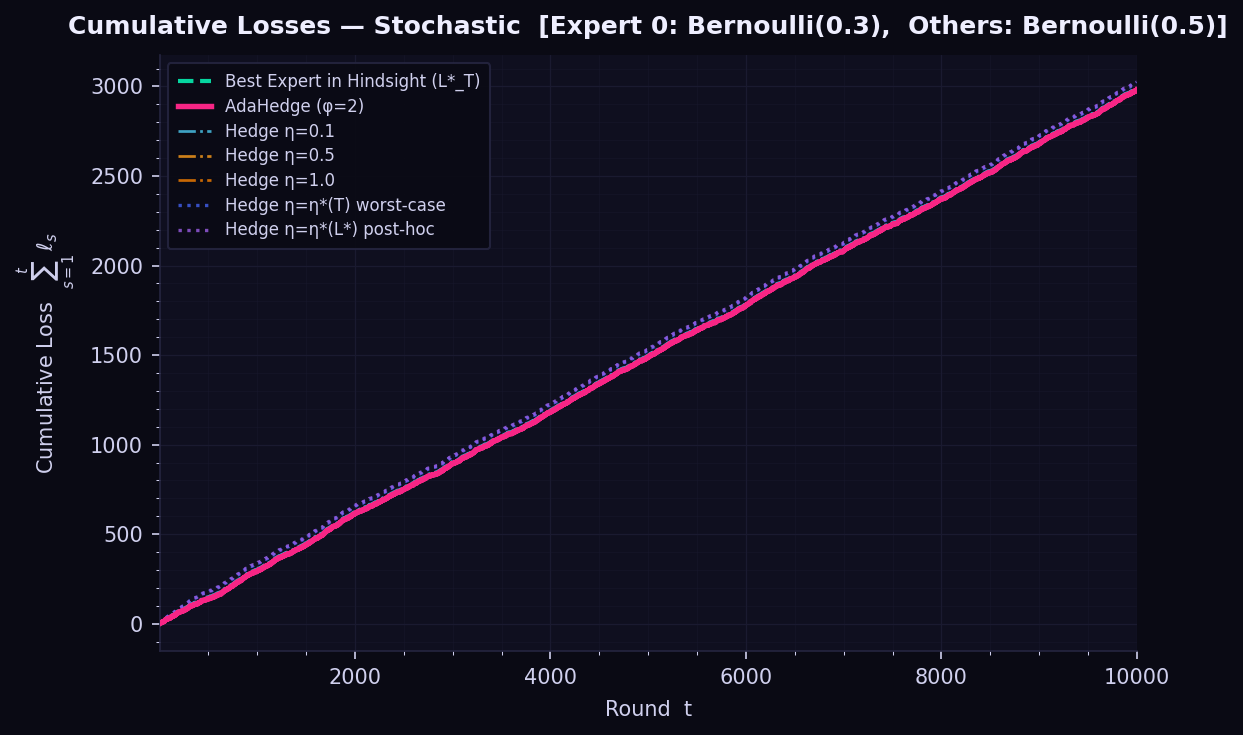
\includegraphics[width=0.48\textwidth]{../Plots/stochastic_cumulative_loss.png}}
  \hspace{1em}
  \subfloat[Cumulative regret\label{fig:stoch_regret}]{%
    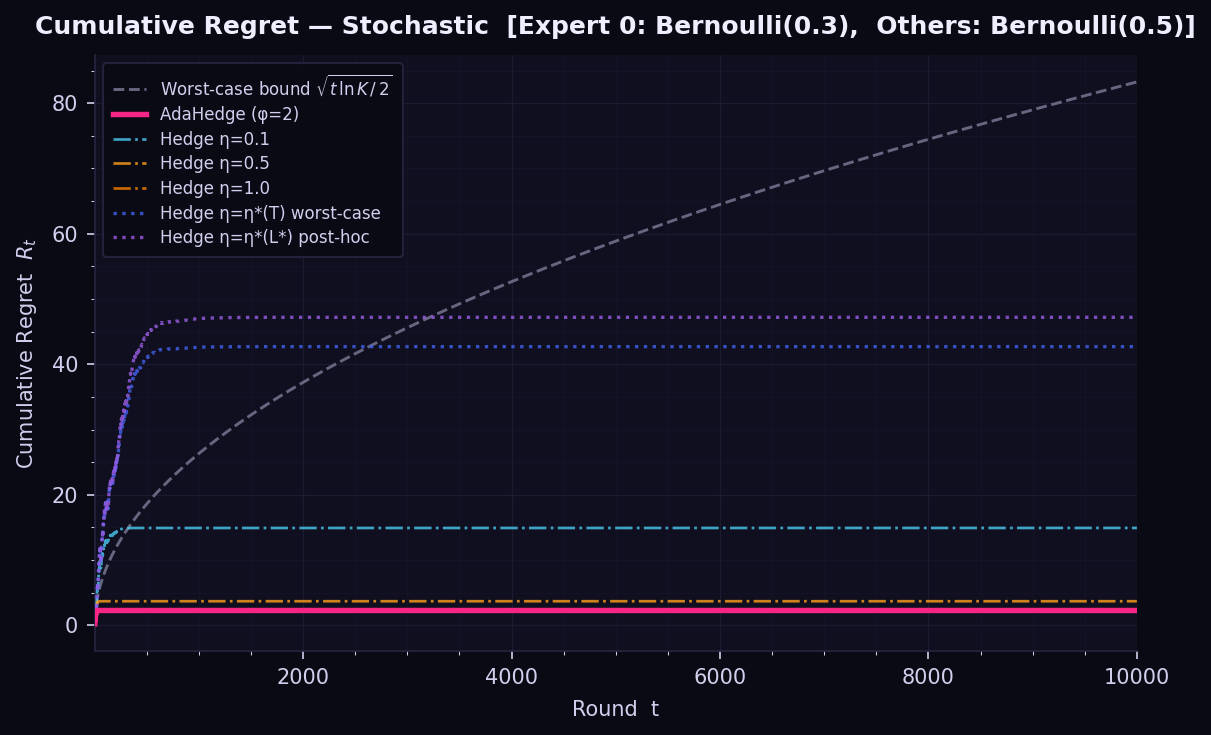
\includegraphics[width=0.48\textwidth]{../Plots/stochastic_cumulative_regret.png}}
  \caption{%
    Stochastic regime: Expert~0 $\sim \mathrm{Bernoulli}(0.3)$,
    Experts~1--3 $\sim \mathrm{Bernoulli}(0.5)$, $T=10{,}000$, $K=4$.
    AdaHedge quickly identifies Expert~0 and achieves near-constant regret.
  }
  \label{fig:stochastic}
\end{figure}

\begin{figure}[h]
  \centering
  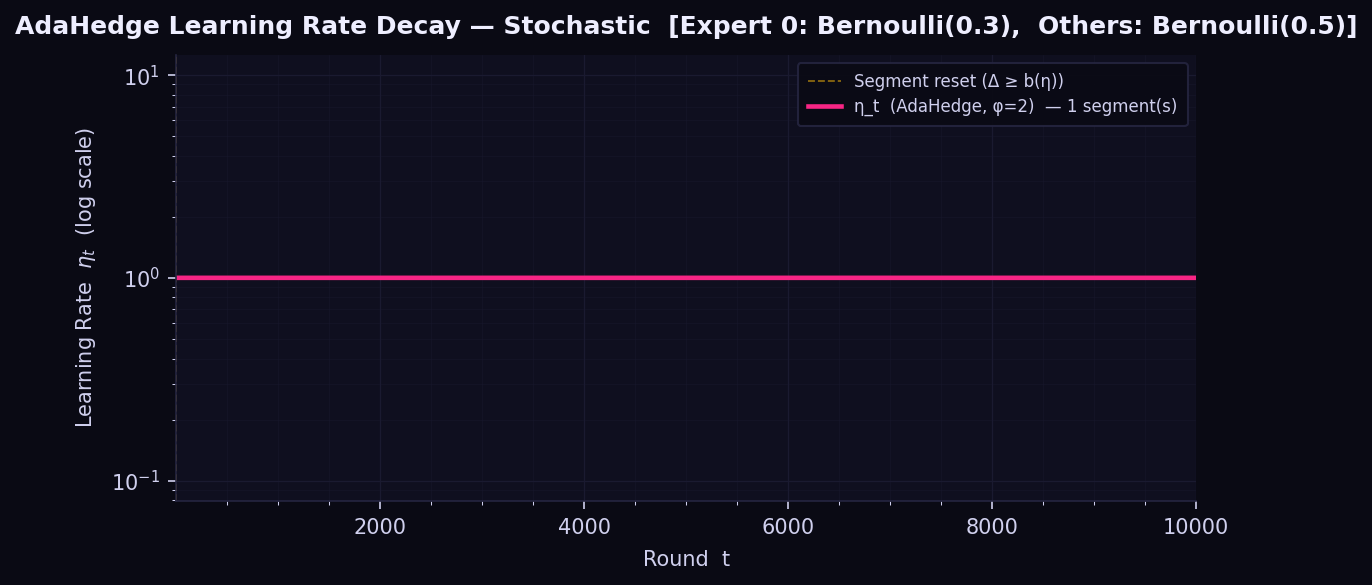
\includegraphics[width=0.58\textwidth]{../Plots/stochastic_learning_rate_decay.png}
  \caption{%
    AdaHedge learning rate decay in the stochastic regime.
    AdaHedge never leaves its initial rate $\eta = 1$. The mixability gap
    never uses up the budget $b(1) \approx 2.19$, so only one segment runs
    for the whole 10{,}000 rounds.
  }
  \label{fig:stoch_eta}
\end{figure}

The stochastic regime is where AdaHedge does best. Expert~0 has a 0.2
advantage in mean loss. By round 10,000 the loss gap between Expert~0 and the
rest is roughly $0.2 \times 10{,}000 = 2{,}000$. Figure~\ref{fig:stoch_regret}
shows AdaHedge's regret levelling off within the first few hundred rounds. It
stays flat after that. The final regret is $2.28$, constant in $T$, just as
Theorem~9 predicts.

Fixed Hedge at $\eta=1.0$ lands on the exact same regret, $2.28$. That is not
a coincidence. AdaHedge never leaves $\eta=1$ in this regime, so with a
single segment its weight updates are identical to fixed Hedge at $\eta=1$.
At the other end, $\eta^*(T)=0.0333$ does much worse, with regret $42.70$.
This rate is tuned for the worst possible sequence over the whole horizon, so
it is too cautious to make use of a 0.2 gap. The post-hoc rate,
$\eta^*(L^*)=0.0301$, does no better even though it gets to look at $\Lstar$
in hindsight: its regret is $47.19$, about $45$ more than AdaHedge.

The learning rate plot (Figure~\ref{fig:stoch_eta}) is just a flat line.
AdaHedge opens one segment and never changes $\eta$ again. With a gap this
big, the leading expert's posterior weight converges to 1 within a few dozen
rounds. By Lemma~\ref{lem:posterior}, the per-round mixability gap then drops
to almost zero almost right away, long before the budget $b(1)\approx 2.19$
runs out. So the algorithm never has a reason to reset.

\subsection{Adversarial Regime}

\begin{figure}[h]
  \centering
  \subfloat[Cumulative losses\label{fig:adv_loss}]{%
    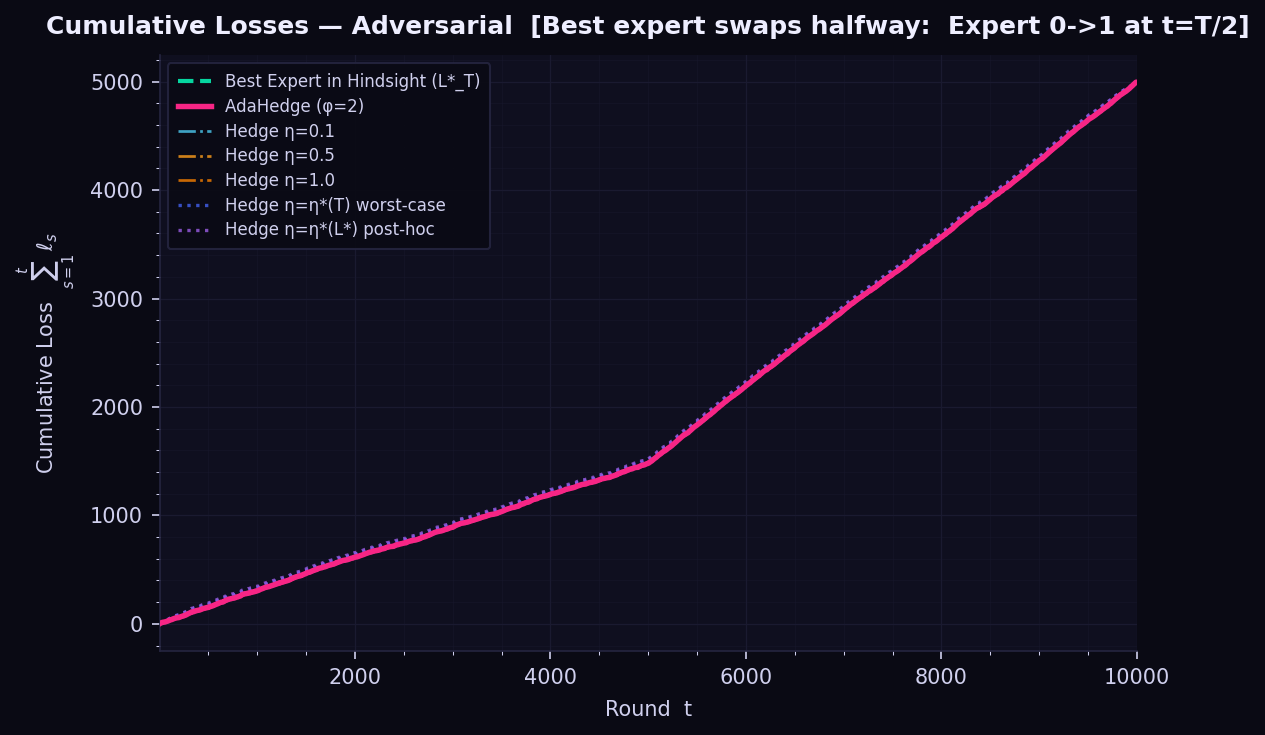
\includegraphics[width=0.48\textwidth]{../Plots/adversarial_cumulative_loss.png}}
  \hspace{1em}
  \subfloat[Cumulative regret\label{fig:adv_regret}]{%
    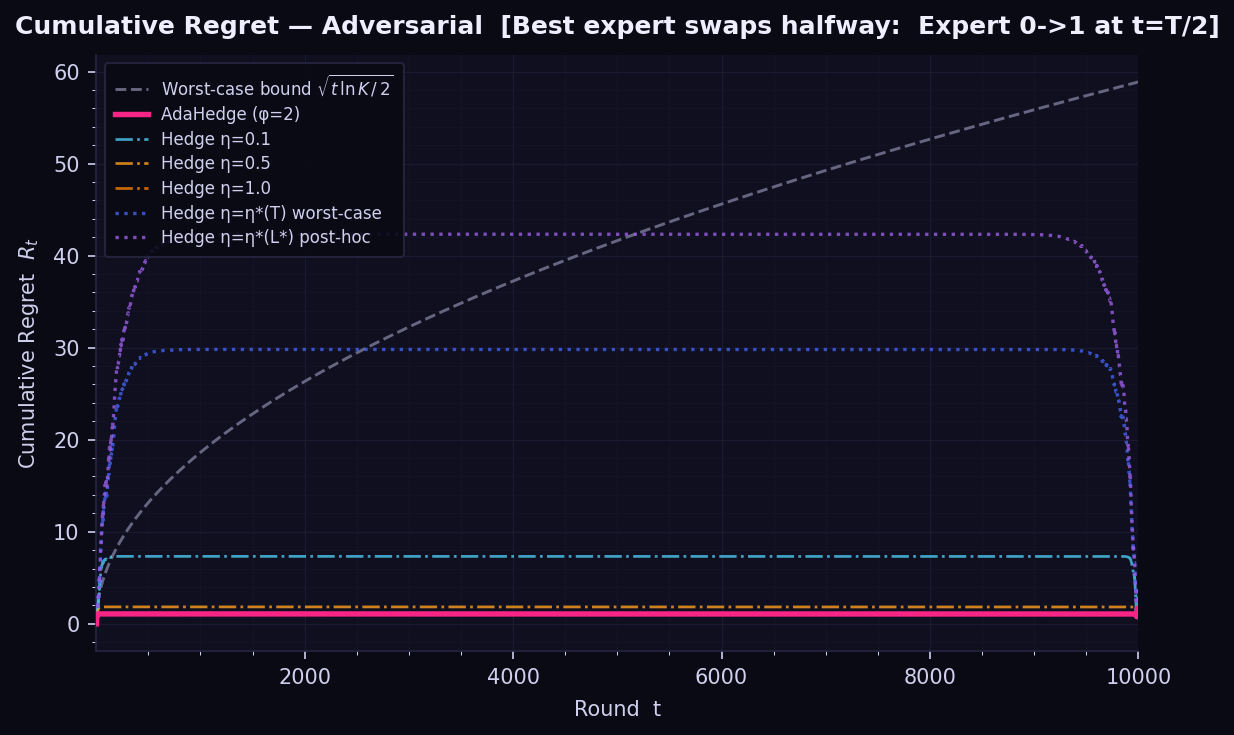
\includegraphics[width=0.48\textwidth]{../Plots/adversarial_cumulative_regret.png}}
  \caption{%
    Adversarial regime: best expert swaps at $t = T/2$.
    $T = 10{,}000$, $K = 2$.  All algorithms show growing regret.
    The dashed reference line is the corrected bound $\sqrt{t\ln K/2} + \ln K$;
    AdaHedge stays below it everywhere.
  }
  \label{fig:adversarial}
\end{figure}

\begin{figure}[h]
  \centering
  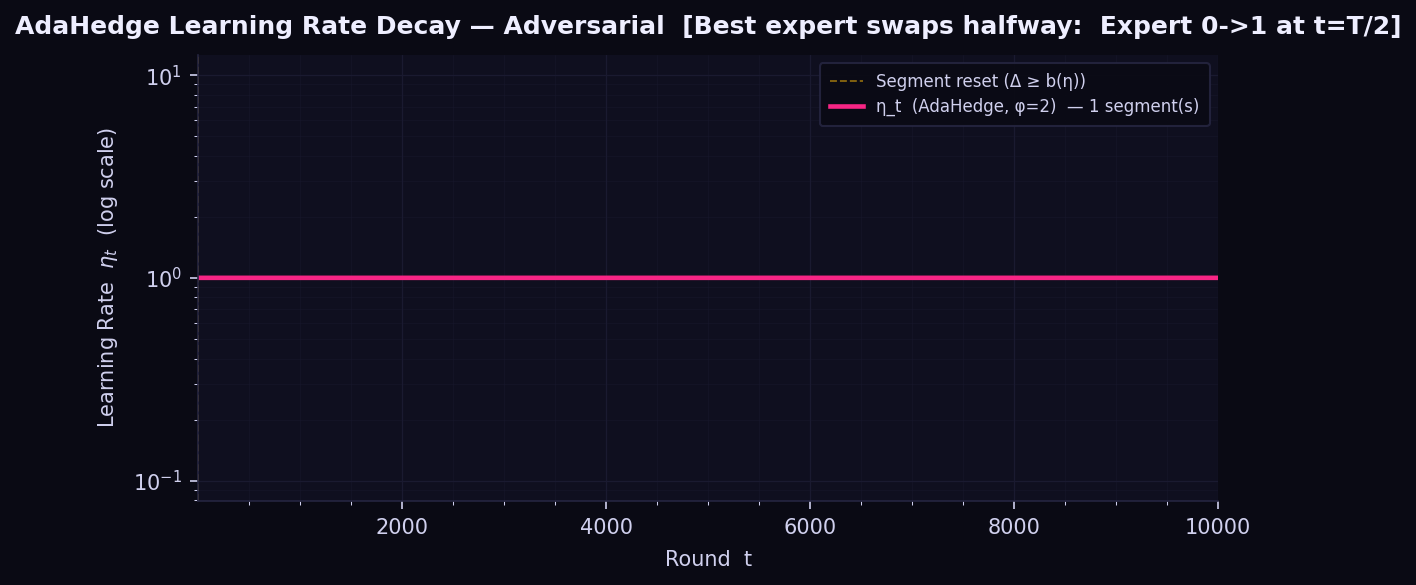
\includegraphics[width=0.58\textwidth]{../Plots/adversarial_learning_rate_decay.png}
  \caption{%
    AdaHedge learning rate in the adversarial regime.  The rate stays near 1
    for most of the run, indicating that the mixability gap is large and the
    algorithm correctly identifies this as a hard sequence.
  }
  \label{fig:adv_eta}
\end{figure}

No algorithm can escape $O(\sqrt{T \ln K})$ regret here in general, and the
results confirm that. Figure~\ref{fig:adv_regret} shows every algorithm's
regret growing over time. The dashed line is the corrected bound
$\sqrt{t\ln K/2}+\ln K$. AdaHedge's curve stays below it at every round and
ends at $1.72$, well inside the more specific Theorem~5 bound of $313.13$ at
$T=10{,}000$.

AdaHedge opens exactly one segment for the whole run. Figure~\ref{fig:adv_eta}
shows the learning rate sitting flat at $1$ the entire time. This is the
right behaviour: in a hard sequence the budget fills up slowly, since
Bernoulli losses rarely come close to the Hoeffding bound on the gap.

There is a kink in the loss curve around round $5{,}000$, visible in
Figure~\ref{fig:adv_loss}. That is where Expert~0's loss rate jumps from 0.3
to 0.7. Any algorithm that had shifted weight onto Expert~0 takes a hit right
there. AdaHedge does not break down, though. At $\eta=1$ its weights stay
spread out enough that probability mass shifts back to Expert~1 within a few
hundred rounds.

Fixed Hedge at $\eta=1.0$ does about as well as AdaHedge here, since both run
at almost the same rate. The slower rates, $\eta=0.1$ and $\eta=0.5$, build up
regret more gently at first but never catch the swap. The worst-case rate
$\eta^*(T)$ is so small it barely tells the two experts apart at all.

\subsection{Low-Gap Stochastic Regime}

\begin{figure}[h]
  \centering
  \subfloat[Cumulative losses\label{fig:lowgap_loss}]{%
    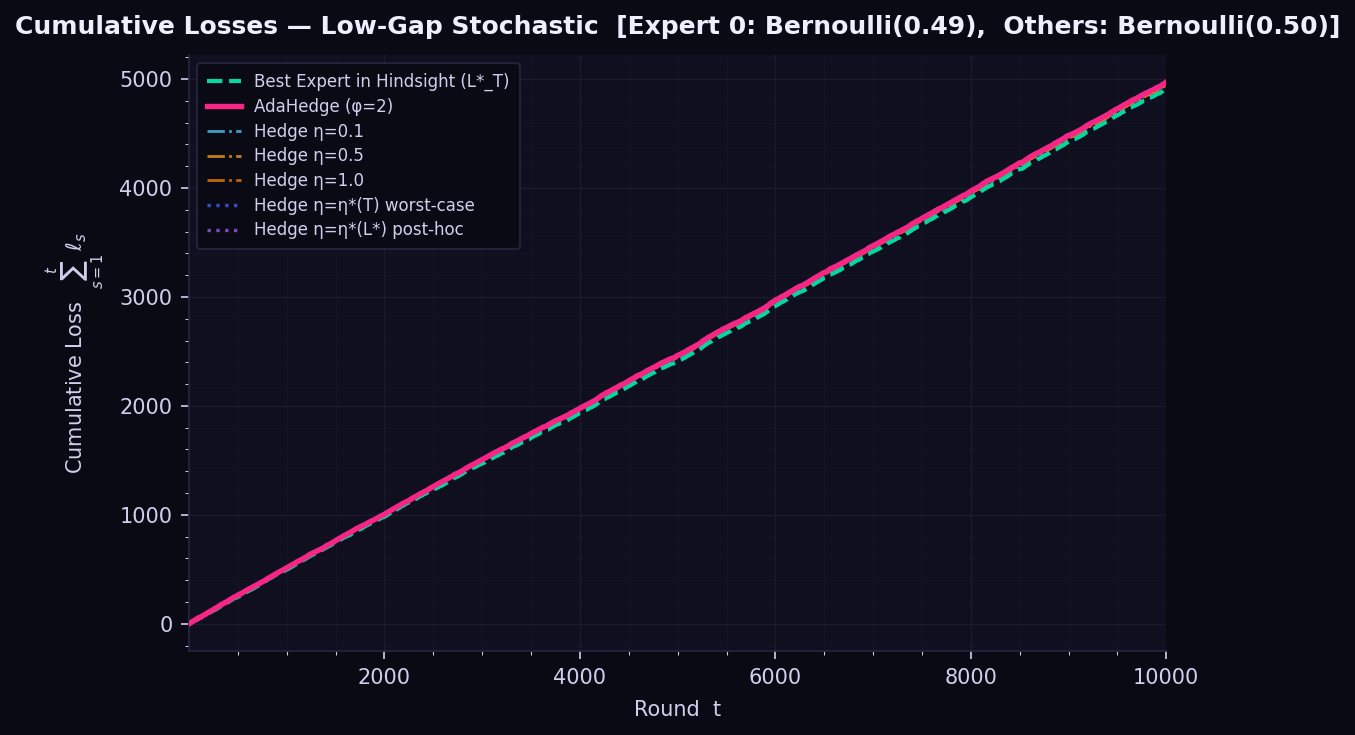
\includegraphics[width=0.48\textwidth]{../Plots/low_gap_cumulative_loss.png}}
  \hspace{1em}
  \subfloat[Cumulative regret\label{fig:lowgap_regret}]{%
    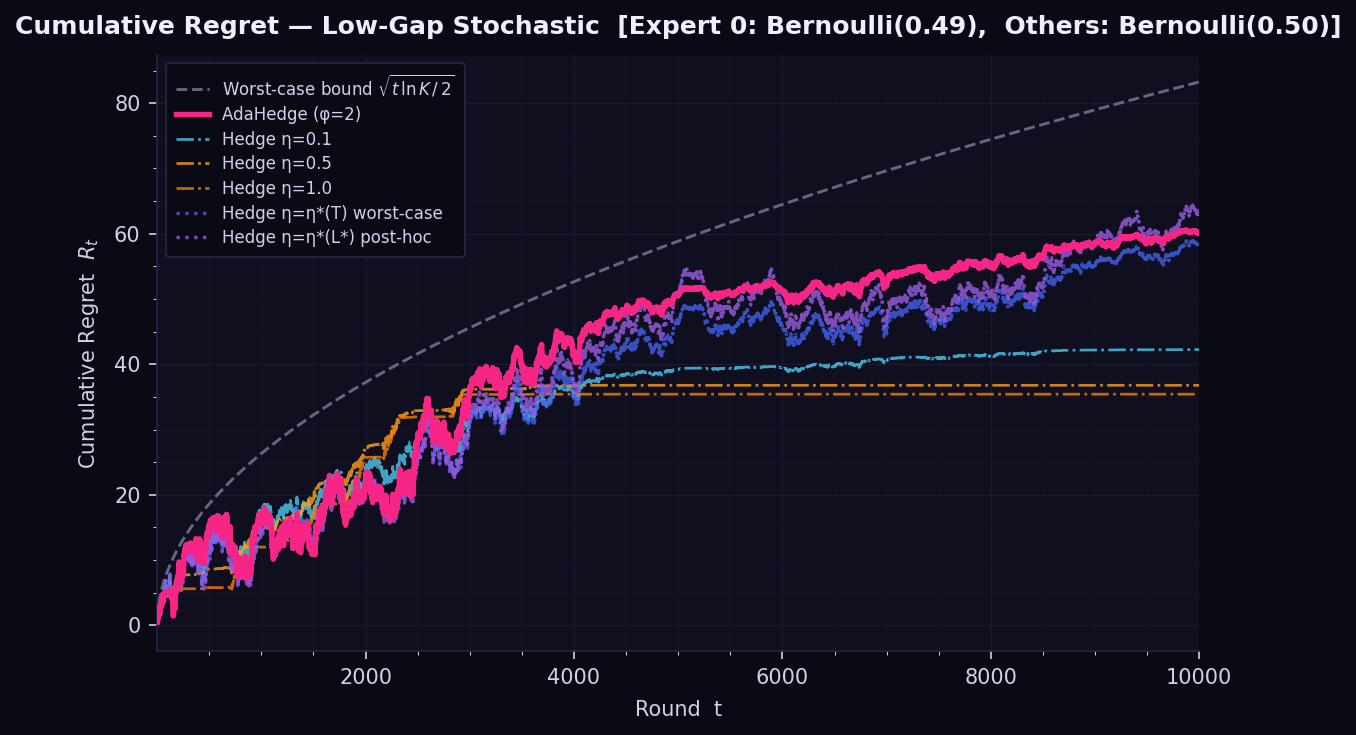
\includegraphics[width=0.48\textwidth]{../Plots/low_gap_cumulative_regret.png}}
  \caption{%
    Low-gap stochastic regime: Expert~0 $\sim \mathrm{Bernoulli}(0.49)$,
    Experts~1--3 $\sim \mathrm{Bernoulli}(0.50)$, $T = 10{,}000$, $K = 4$.
    AdaHedge needs five segments to settle on a rate. Several fixed-$\eta$
    baselines end up with lower regret on this run. AdaHedge still stays
    well inside its theoretical guarantee (Theorem~5).
  }
  \label{fig:lowgap}
\end{figure}

\begin{figure}[h]
  \centering
  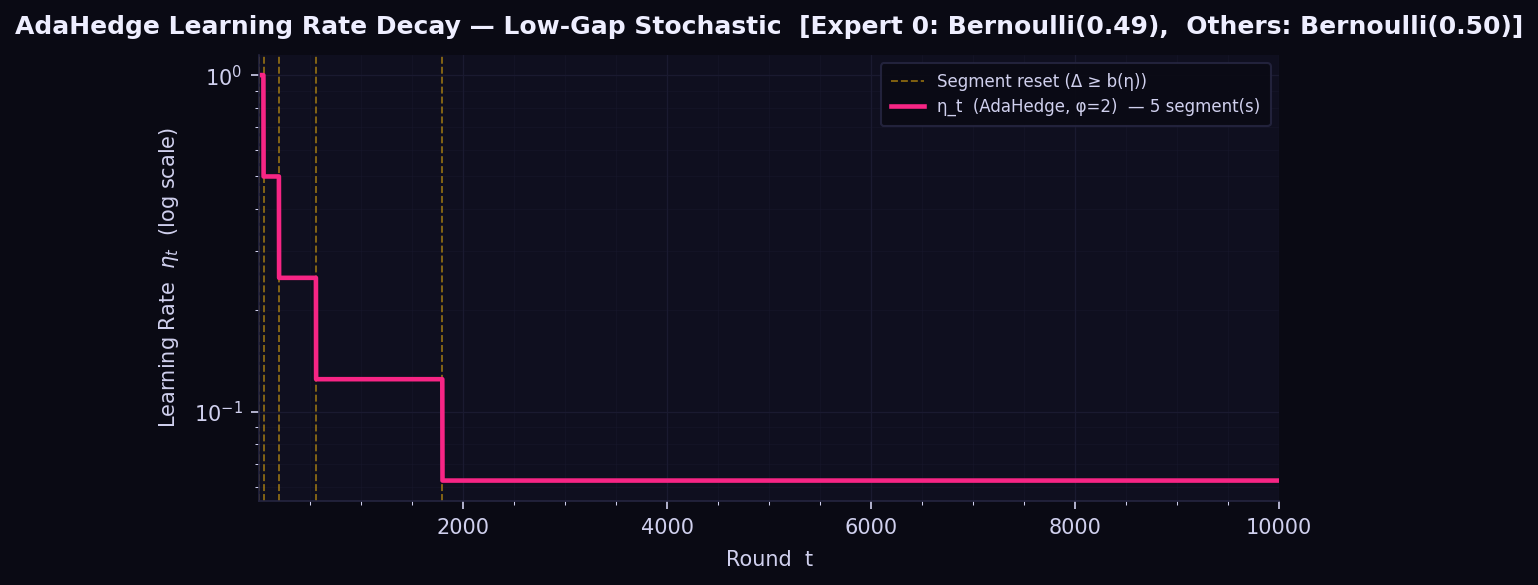
\includegraphics[width=0.58\textwidth]{../Plots/low_gap_learning_rate_decay.png}
  \caption{%
    AdaHedge learning rate in the low-gap regime.  The rate decays more slowly
    than in the stochastic case, reflecting that Expert~0 is harder to identify
    when the gap is only 0.01.
  }
  \label{fig:lowgap_eta}
\end{figure}

The low-gap regime is the most useful of the three. It shows the gap between
an adaptive method and a fixed one, on a problem that is easy in theory but
hard to spot in practice.

Figure~\ref{fig:lowgap_regret} shows the worst-case-tuned rates struggling the
most. $\eta^*(T)=0.0333$ gets regret $58.17$, and $\eta^*(L^*)=0.0235$ gets
$62.91$. Both are almost blind to a gap this small, since they were tuned for
a much harder sequence. What is a bit surprising is that the simple, aggressive
rates do better here. $\eta=1.0$ gets the lowest regret of all six methods on
this run, $35.42$, followed by $\eta=0.5$ at $36.78$ and $\eta=0.1$ at $42.25$.

AdaHedge's final regret is $60.06$. That is worse than every fixed rate except
the post-hoc one, and even a little worse than the worst-case rate
$\eta^*(T)$. This does not break the theory. Theorem~5 only promises AdaHedge
stays under $440.49$ here, and $60.06$ is well inside that. Here is what
happens: with a gap this small ($\alpha=0.01$), AdaHedge spends its first
five segments resetting to uniform weights and starting over. By the time it
settles on $\eta=0.0625$, that rate is already more careful than even the
$\eta=0.1$ baseline. It is too careful to catch a $0.01$ gap over the roughly
$8{,}200$ rounds that are left.

The lesson here is simple. A constant-regret guarantee is about the worst
case, no matter how big its constant is. It does not promise a win against
every other method on one specific run. The constant behind Theorem~9 also
grows fast as $\alpha$ shrinks: it scales roughly as $O(1/\alpha^2)$, through
the number of segments $m^*$, which itself grows like $\log_\phi(1/\alpha^2)$.
Here $\alpha=0.01$ is twenty times smaller than the $\alpha=0.2$ from the
stochastic regime, so this constant is much bigger too.

Figure~\ref{fig:lowgap_eta} shows exactly this. AdaHedge walks through five
segments, $\eta$ going $1, 0.5, 0.25, 0.125$, then $0.0625$. All five changes
happen in the first $1{,}800$ rounds. After that the rate never moves again
for the remaining $8{,}200$ rounds. The gap is small, so the mixability gap
per round shrinks more slowly than in the stochastic case. That means more
resets, and more time, before the algorithm lands on a rate that stops using
up its budget.

\subsection{Summary of Results}

Table~\ref{tab:summary} collects the final cumulative regret for AdaHedge and
the five Hedge variants across all three regimes.

\begin{table}[h]
  \centering
  \small
  \caption{Final cumulative regret at $t = 10{,}000$, re-run directly from the
  submitted code with seed 777 (exact console output, not read off a plot).
  $K=4$ in the stochastic and low-gap columns, $K=2$ in the adversarial column.}
  \label{tab:summary}
  \begin{tabular}{lrrr}
    \toprule
    Algorithm & Stochastic & Adversarial & Low-gap \\
    \midrule
    AdaHedge ($\phi = 2$)              & $2.28$  & $1.72$ & $60.06$ \\
    Hedge $\eta = 0.1$                  & $14.92$ & $3.67$ & $42.25$ \\
    Hedge $\eta = 0.5$                  & $3.70$  & $2.36$ & $36.78$ \\
    Hedge $\eta = 1.0$                  & $2.28$  & $1.72$ & $35.42$ \\
    Hedge $\eta^*(T)$, worst-case       & $42.70$ & $4.06$ & $58.17$ \\
    Hedge $\eta^*(L^*)$, post-hoc       & $47.19$ & $4.10$ & $62.91$ \\
    AdaHedge bound (Thm.~5, at $t=T$)   & $343.98$ & $313.13$ & $440.49$ \\
    Fixed-Hedge envelope $\sqrt{T\ln K/2}$ & $83.26$ & $58.87$ & $83.26$ \\
    \bottomrule
  \end{tabular}
\end{table}

A few patterns stand out. No single fixed rate works well in all three
regimes. The worst-case rate $\eta^*(T)$ does fine in the adversarial case,
since it was built for exactly that kind of sequence, but it is one of the
worst performers in the two stochastic regimes. On the other hand, $\eta=1.0$
is the best fixed rate in both stochastic regimes, but it loses to the more
careful rates in the adversarial case.

AdaHedge does not need to know which regime it is in ahead of time. In the
stochastic regime, and in the adversarial swap too, it matches the best fixed
rate exactly, without ever seeing the sequence in advance. The low-gap regime
breaks this pattern on this specific run: several fixed rates beat AdaHedge
here, even though its theoretical bound (Theorem~5) still holds with plenty
of room to spare. This is the clearest example in this report that a
constant-regret guarantee is a worst-case statement, not a promise to win
every comparison.

The post-hoc rate $\eta^*(L^*)$ needs to know $\Lstar$ before the game
starts, which is not a fair advantage for a real algorithm to have. AdaHedge
still beats it clearly in the stochastic regime ($2.28$ vs $47.19$) and stays
close behind it in the adversarial regime ($1.72$ vs $4.10$). In the low-gap
regime, AdaHedge is the only method that beats the post-hoc rate at all
($60.06$ vs $62.91$), though it still loses to the plainer fixed rates
$\eta=1.0, 0.5, 0.1$ there. So AdaHedge usually keeps up with a rate that
gets to cheat, without ever being told $\Lstar$ or $T$ in advance. It just
does not guarantee a win every single time.

% =============================================================
\section*{References}
\addcontentsline{toc}{section}{References}

\small
\begin{enumerate}[label={[\arabic*]}, leftmargin=2em, itemsep=2pt, parsep=0pt, topsep=4pt]
  \item Tim van Erven, Peter D.\ Gr\"{u}nwald, Wouter M.\ Koolen, and Steven de Rooij.
        \textit{Adaptive Hedge}.
        NeurIPS 2011.
        \texttt{https://arxiv.org/abs/1110.1877}
  \item Nicol\`{o} Cesa-Bianchi and G\'{a}bor Lugosi.
        \textit{Prediction, Learning, and Games}.
        Cambridge University Press, 2006.
  \item Yoav Freund and Robert E.\ Schapire.
        A decision-theoretic generalization of on-line learning and an application to boosting.
        \textit{Journal of Computer and System Sciences}, 55(1):119--139, 1997.
\end{enumerate}

% =============================================================
\end{document}
